\label{sec:cnninterrupt}
The idea of interruption is introduced for dynamic multi-thread scheduling. This section details the implementation of our \textbf{Virtual Instrcution Interruption}. \Cref{fig:interDPR} illustrates the idea of interruption to full utilize the hardware resources.


\begin{figure}
	\centering
	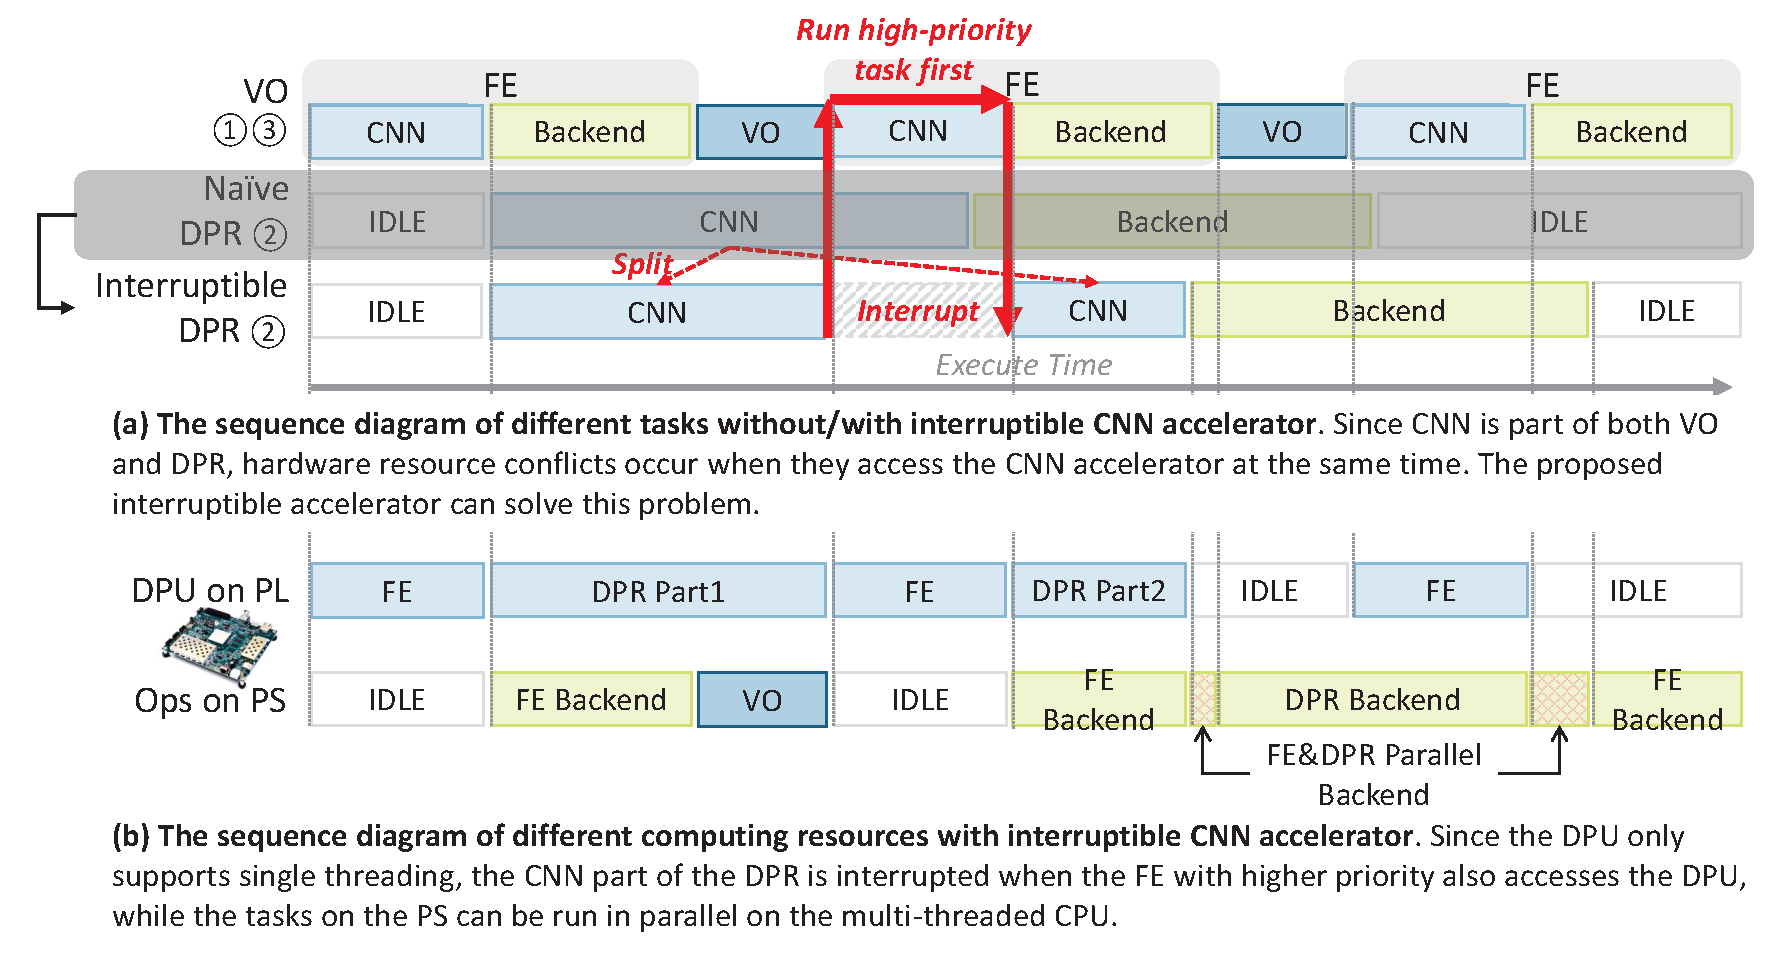
\includegraphics[width=0.99\linewidth]{fig/interDPR.eps}
	\caption{Interruption to solve the hardware resources conflicts.  When a high-priority task (VO) is started before the low-priority task (PR) is completed, the CNN accelerator backupes the status of PR to memory, and processes the VO task. When the high-priority task is completed, the low-priority task resumes and continues.
    }
	\label{fig:interDPR}
\end{figure}

\subsection{How To Interrupt: Virtual Instruction}
\label{sec:howinter}

In order to support multi-thread scheduling, interruption has been introduced in CPU for decades. In CPU, when a high-priority task requires a interruption, the hardware or the interrupt handler software would backup the registers to main memory, and after the high-priority task, the backed-up registers will be recovered to CPU hardware. This CPU-like interruption can switch the between tasks with low latency.

However, the CPU-like interruption would back-up all the on-chip registers to main memory. In CPU, there are tens of registers, and the backed-up data is around 1 KB. In CNN accelerators, there are hundreds of KB ~ several MB on-chip cache \cite{qiu2016going, yu2018instruction}. The cost of data transfer in the CNN accelerator is much higher than that of CPU if all the on-chip cache is backed up and recovered.

We propose the \textbf{Virtual Instrcution Interruption} method. The low-priority maintain the executing status itself rather than the hardware or the interrupt handler. Only the cache which is still needed in future execution will be backed up and restored.

The virtual instructions, which contain the back-up and recovery instructions, are generated at compiling stage, together with the normal instructions. For backup instructions, the corresponding input data and weights are still stored in DDR. There is no need to backup the input buffer and weight buffer, and only the intermediate data and the final output results are needed to be backed up. For recovery instructions, the weights and input data for future calculation, as well as the backed-up intermediate data, are needed to restored from DDR to on-chip cache.

There is a field in instruction set to indicate if a instruction a virtual instruction. If no interruption occurs, virtual instructions will be skipped and discarded, which can ensure the efficiency of execution without interruption.

\subsection{ Where To Interrupt: After Save/CALC\_F }
\label{sec:whereinter}

There are three kinds of instruction in the a instruction-driven accelerator: LOAD, CALC and SAVE. The instruction description and the back-up/recovery data for interruption after each kind of instruction is list in \Cref{fig:normal_instr} and \Cref{tab:instr}.

\begin{figure}[h]
	\centering
	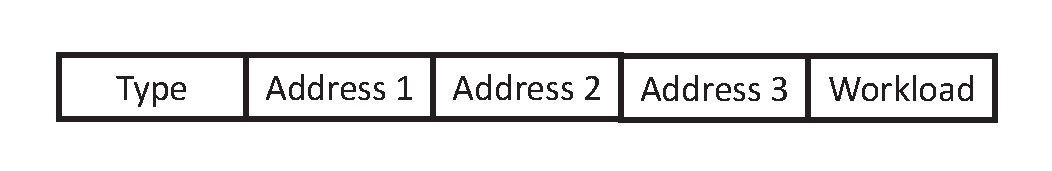
\includegraphics[width=0.9\linewidth]{fig/normal_instr.eps}
	\caption{The extended insrtuction set for virtual instruction interrupt }
	\label{fig:normal_instr}
\end{figure}


\begin{table*}[t]
	\centering
	\caption{Description for the basic instructions.}
% Table generated by Excel2LaTeX from sheet 'Sheet3'
\begin{tabular}{|p{2.7em}|p{3.4em}|p{12.3em}|p{4.2em}|p{4.6em}|p{4.2em}|p{4.2em}||p{4.2em}|p{4.2em}|}
	\hline
	\multicolumn{1}{|c|}{Category} & \multicolumn{1}{c|}{Type} & \multicolumn{1}{c|}{Description} & \multicolumn{1}{c|}{Address 1} & \multicolumn{1}{c|}{Address 2} & \multicolumn{1}{c|}{Address 3} & \multicolumn{1}{c||}{Workload} & \multicolumn{1}{c|}{Backups} & \multicolumn{1}{c|}{Recovery $^1$} \bigstrut\\
	\hline
	\multirow{2}[4]{*}{LOAD} & LOAD\_W & Load weights/bias from DDR to on chip weight buffer. & Off-chip Addr & Weights-buffer Addr & -     & Data  Length & -     & Weight / Inputdata \bigstrut\\
	\cline{2-9}\multicolumn{1}{|c|}{} & LOAD\_D & Load input data from DDR to on-chip data buffer. & Off-chip Addr & Data-buffer Addr & -     & Data  Length & -     & Weight / Inputdata \bigstrut\\
	\hline
	\multirow{2}[4]{*}{CALC} & CALC\_I & Calculate intermediate results for some output channels from partial  input channels. & Input  Data Addr & Intermediate Data Addr & Weight Addr & Calc Size & Previous final results / Intemediate data  & Weight / Inputdata /  intemediate data \bigstrut\\
	\cline{2-9}\multicolumn{1}{|c|}{} & CALC\_F & Calculate the results for some output channels from all input channels. The pooling, bias-adding and elementwise operations are operated in this instructions. & Input  Data Addr & Output  Data Addr & Weight Addr & Calc Size & Finial results & Weight / Inputdata \bigstrut\\
	\hline
	SAVE  & SAVE  & Save the results from on-chip data buffer to DDR. & Off-chip Addr & Data-buffer Addr & -     & Data  Length & -     & Weight / Inputdata \bigstrut\\
	\hline
	\end{tabular}%
	
	\label{tab:instr}%
  \end{table*}%


\subsubsection{LOAD\_W / LOAD\_D }
When interrupt after the LOAD instruction. The newly loaded data would inmediately flushed when running the high-level CNN, leading to bandwidth waste.

\subsubsection{CALC\_I} 
When interrupt after CALC\_I, the previous calculated yet not-saved finial results, which are generated by previous CALC\_F should be saved to DDR. The intermediate data with current CALC\_I should also be send to DDR for further use. At the Recovery stage, the intermediate data should be fetch from DDR. The data handling of intemediate results lead to extra bandwidth requirements.


\subsubsection{CALC\_F}
When interrupt after CALC\_F, there is no need to backup and recovery intermediate results. Although it is necessary to backup the final results which are generated by previous CALC yet not stored to DDR, these results will stored in DDR by the subsequent normal SAVE instruction. If the interrupt status can be recorded, we can modify the address and worklaod when executing the subsequent normal SAVE instruction. So that we can avoid the duplicate transporting of results. The state records and modifications to normal SAVE instruction will be introduced in following subsections.

\subsubsection{SAVE}
When interrupt after SAVE, there is no need to back up any data. The overhead of interruption is only the data transfer of input data and weights from DDR to on-chip cache.

We want to minimize the cost for interruption. We make the scheduling of low-priority CNN interruptible after the SAVE or CACL\_F instructions, introducing extra data transfer to recovery input data and weights without any excess backup data transfer.

The extra virtual instructions also need extra bandwidth for instruction fetch even though they are not executed. The instruction number of CALC\_I is tens of times of that of SAVE/CALC\_F. If the network can be interrupted after each CALC\_I, the rapidly increasing virtual instructions would reduce the system performance.

\subsection{ Instruction Improvement }
\label{sec:virtualinstr}

We extend the instruction set illustrate in \Cref{fig:normal_instr}. To field are added: 1) Virtual and 2) SaveID, as shown in  \Cref{fig:virtual_instr}.

\begin{figure}[h]
	\centering
	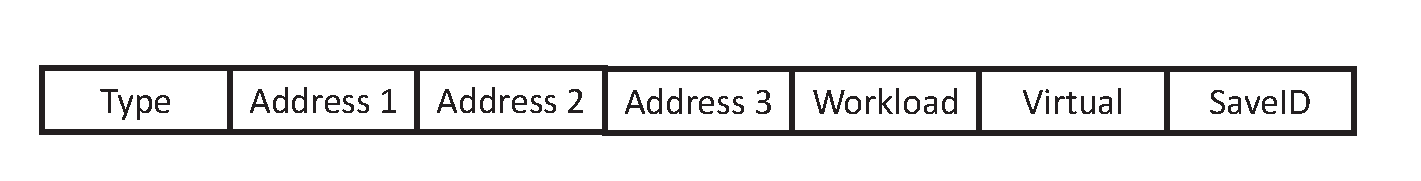
\includegraphics[width=0.9\linewidth]{fig/virtual_instr.eps}
	\caption{The basic structure of a instruction }
	\label{fig:virtual_instr}
\end{figure}

\subsubsection{ Virtual Filed}

Three value can be set to Virtual Filed:
\begin{itemize}
    \item[2'b00] indicates this instruction is not virtual, should always executed.
    \item[2'b01] indicates this instruction is the SAVE instruction for backup. When interruption occurs, the high-priority network will start after this instruction.
    \item[2'b10] indicates this instruction is the LAOD instruction for recovery. The corresponding instructions will executed after the interruption. 
\end{itemize}

\subsubsection{ SaveID Filed }

SaveID links LAOD/CALC instructions with corresponding SAVE instruction. SaveID of each not virtual SAVE instrcution differs. The LOAD/CALC instructions have the same SaveID as a SAVE instruction, if the genterated output data of the LOAD/CALC are stored to DDR by the SAVE instruction. 

We consider the LOAD/CALC instructions serve for one CALC\_F instrcution as a \textbf{CalcBlob}. Each CalcBlob has one CALC\_F instrcution, and ends up with this CALC\_F instrcution. The SaveID for a CalcBlob is the same as its CALC\_F instrcution.
One SAVE instruction may serve for one CalcBlob ( \textbf{Single Blob Save}, illustrated in \Cref{fig:singlesave} ) or several CalcBlobs (\textbf{Multiple Blob Save}, illustrated in \Cref{fig:multisave}).

For Single Blob Save, no virtual SAVE is added. The high-priority network can start after the nomal SAVE is completed. The virtual LOAD instructions for data recovery are generated after the normal SAVE, and executed after the high-priority network. The execution timeline is shown in \Cref{fig:intersinglesave}.

For Multiple Blob Save, virtual SAVE and LOAD instructions are generated after the CALC\_F of each CalcBlob. When the interrupt request occurs during the CalcBlob, the virtual SAVE instruction will be executed before the high-priority network starts. Virtual LOAD instructions are executed for data recovery. The subsequent nomal SAVE instruction with the same SaveID as the CalcBlob will be modified to avoid duplicate output data transfer. The execution timeline is shown in \Cref{fig:intermultisave}.




\begin{figure*}[t]
	\begin{minipage}[t]{0.2\linewidth}  
	\centering
	\subfigure[One Save for Single CACL/LOAD.] {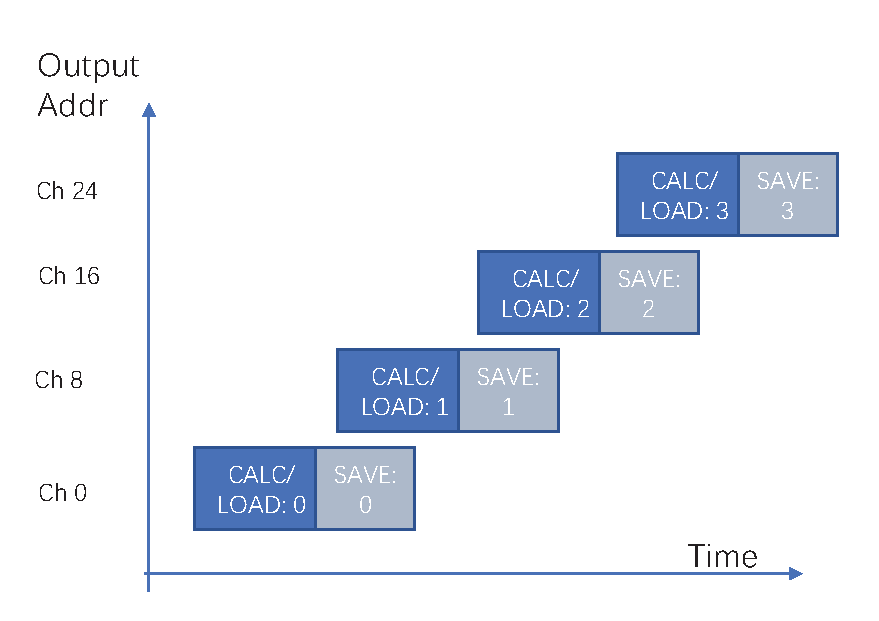
\includegraphics[width=0.9\linewidth]{fig/singlesave.eps}\label{fig:singlesave}}
	\end{minipage}
	\begin{minipage}[t]{0.2\linewidth}  
	\centering  
	\subfigure[One Save for Multiple CACL/LOAD.] {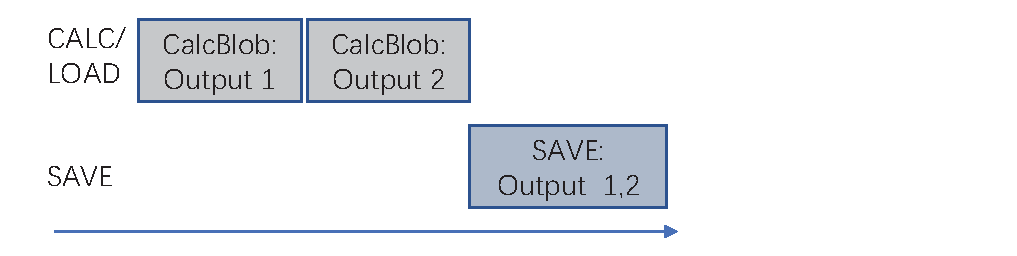
\includegraphics[width=0.9\linewidth]{fig/multisave.eps}\label{fig:multisave}} 
	\end{minipage}
	\begin{minipage}[t]{0.3\linewidth}  
	\centering  
	\subfigure[Interrupt for \Cref{fig:singlesave} ] {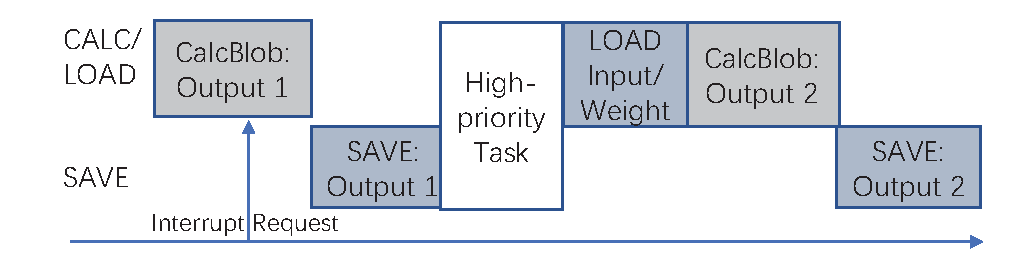
\includegraphics[width=0.9\linewidth]{fig/intersingle.eps}\label{fig:intersinglesave}} 
	\end{minipage}
	\begin{minipage}[t]{0.3\linewidth}  
	\centering  
	\subfigure[Interrupt for \Cref{fig:multisave}] {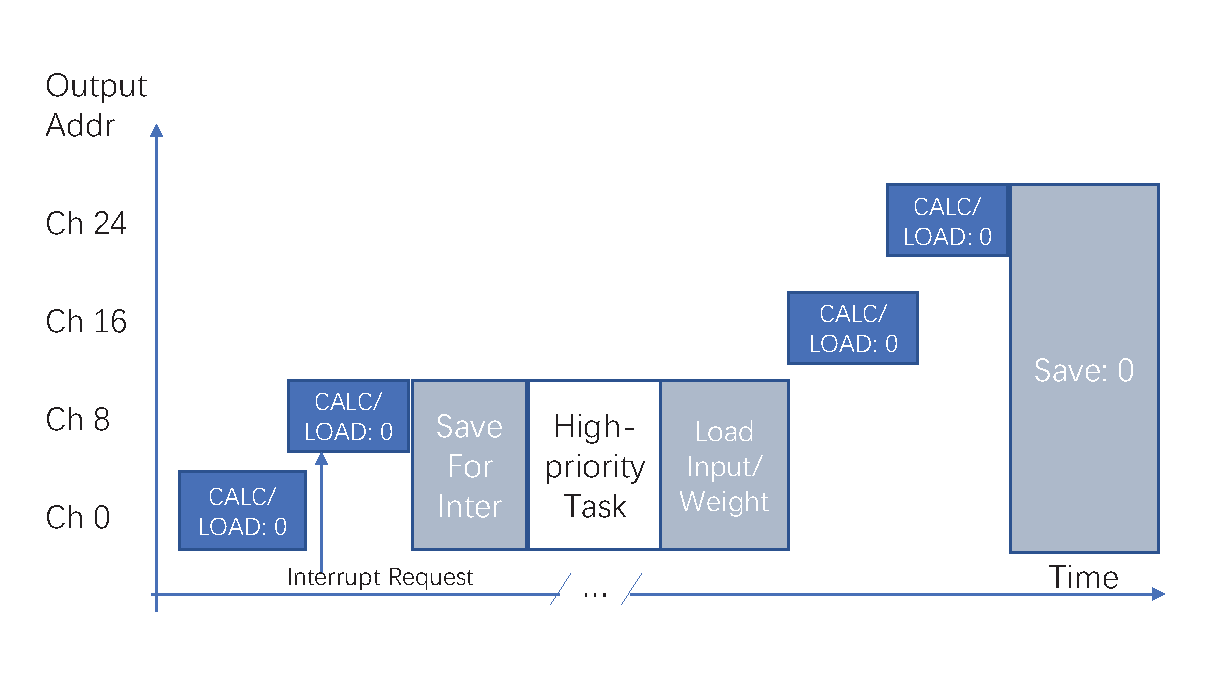
\includegraphics[width=0.9\linewidth]{fig/intermulti.eps}\label{fig:intermultisave}} 
	\end{minipage}
	\caption{ Scheduling Illustration
%   (d) find a single intra-robot loop closure which (c) and (d) cannot find, so that the result is better than (c) and (e).
  }
\label{fig:dslamresult}
\end{figure*}


\subsection{ Instruction Arrangement Unit (IAU) }

A specific hardware module called Instruction Arrangement Unit (IAU) is designed to handle the computing requirements from different tasks. The IAU monitors the interrupt states, and generates a simple instruction sequence dynamically. The decoder, controller, processing elements in the CNN accelerator do not need to know the interrupt states, and operate the instructions provided by IAU as a simple CNN.
